\section{Conclusion}

\begin{frame}{Summary \& Outlook}
	\begin{itemize}
		\item
		allocation:
		partition of items amongst agents

		\item
		bundles valued using submodular valuation functions
		\begin{itemize}
			\item
			diminishing returns
		\end{itemize}

		\item
		Nash social welfare:
		weighted geometric mean of valuations

		\item
		approximation factor independent from \(m\)?

		\item
		simple, repeated matching fails because of missing foresight

		\item
		\RepReMatch:
		\(2n (\log n + 3)\)-approximative
		\begin{description}
			\item[Phase \phasei]
			finding enough outstanding items

			\item[Phase \phaseii]
			assigning remaining item

			\item[Phase \phaseiii]
			assigning outstanding items
		\end{description}
	\end{itemize}
	\beamerimage at (13cm, 5.50cm) {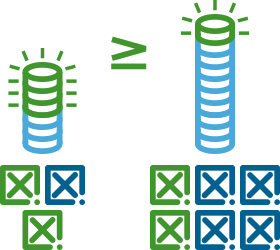
\includegraphics[height=1.45cm]{img/diminishingreturns}};
	\beamerimage at (13cm, 3.75cm) {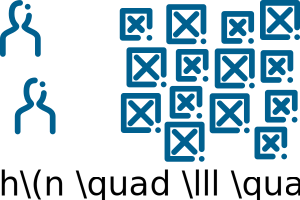
\includegraphics[height=1.45cm]{img/nvsm}};
	\beamerimage at (13cm, 2.00cm) {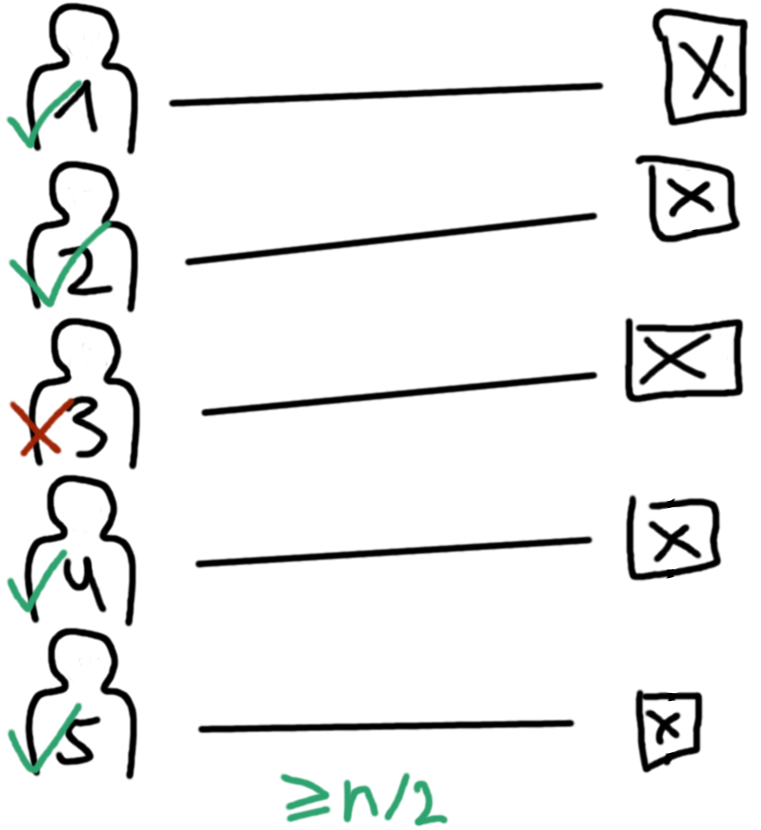
\includegraphics[height=1.45cm]{img/outstanding_1}};
	\beamerimage at (13cm, 0.25cm) {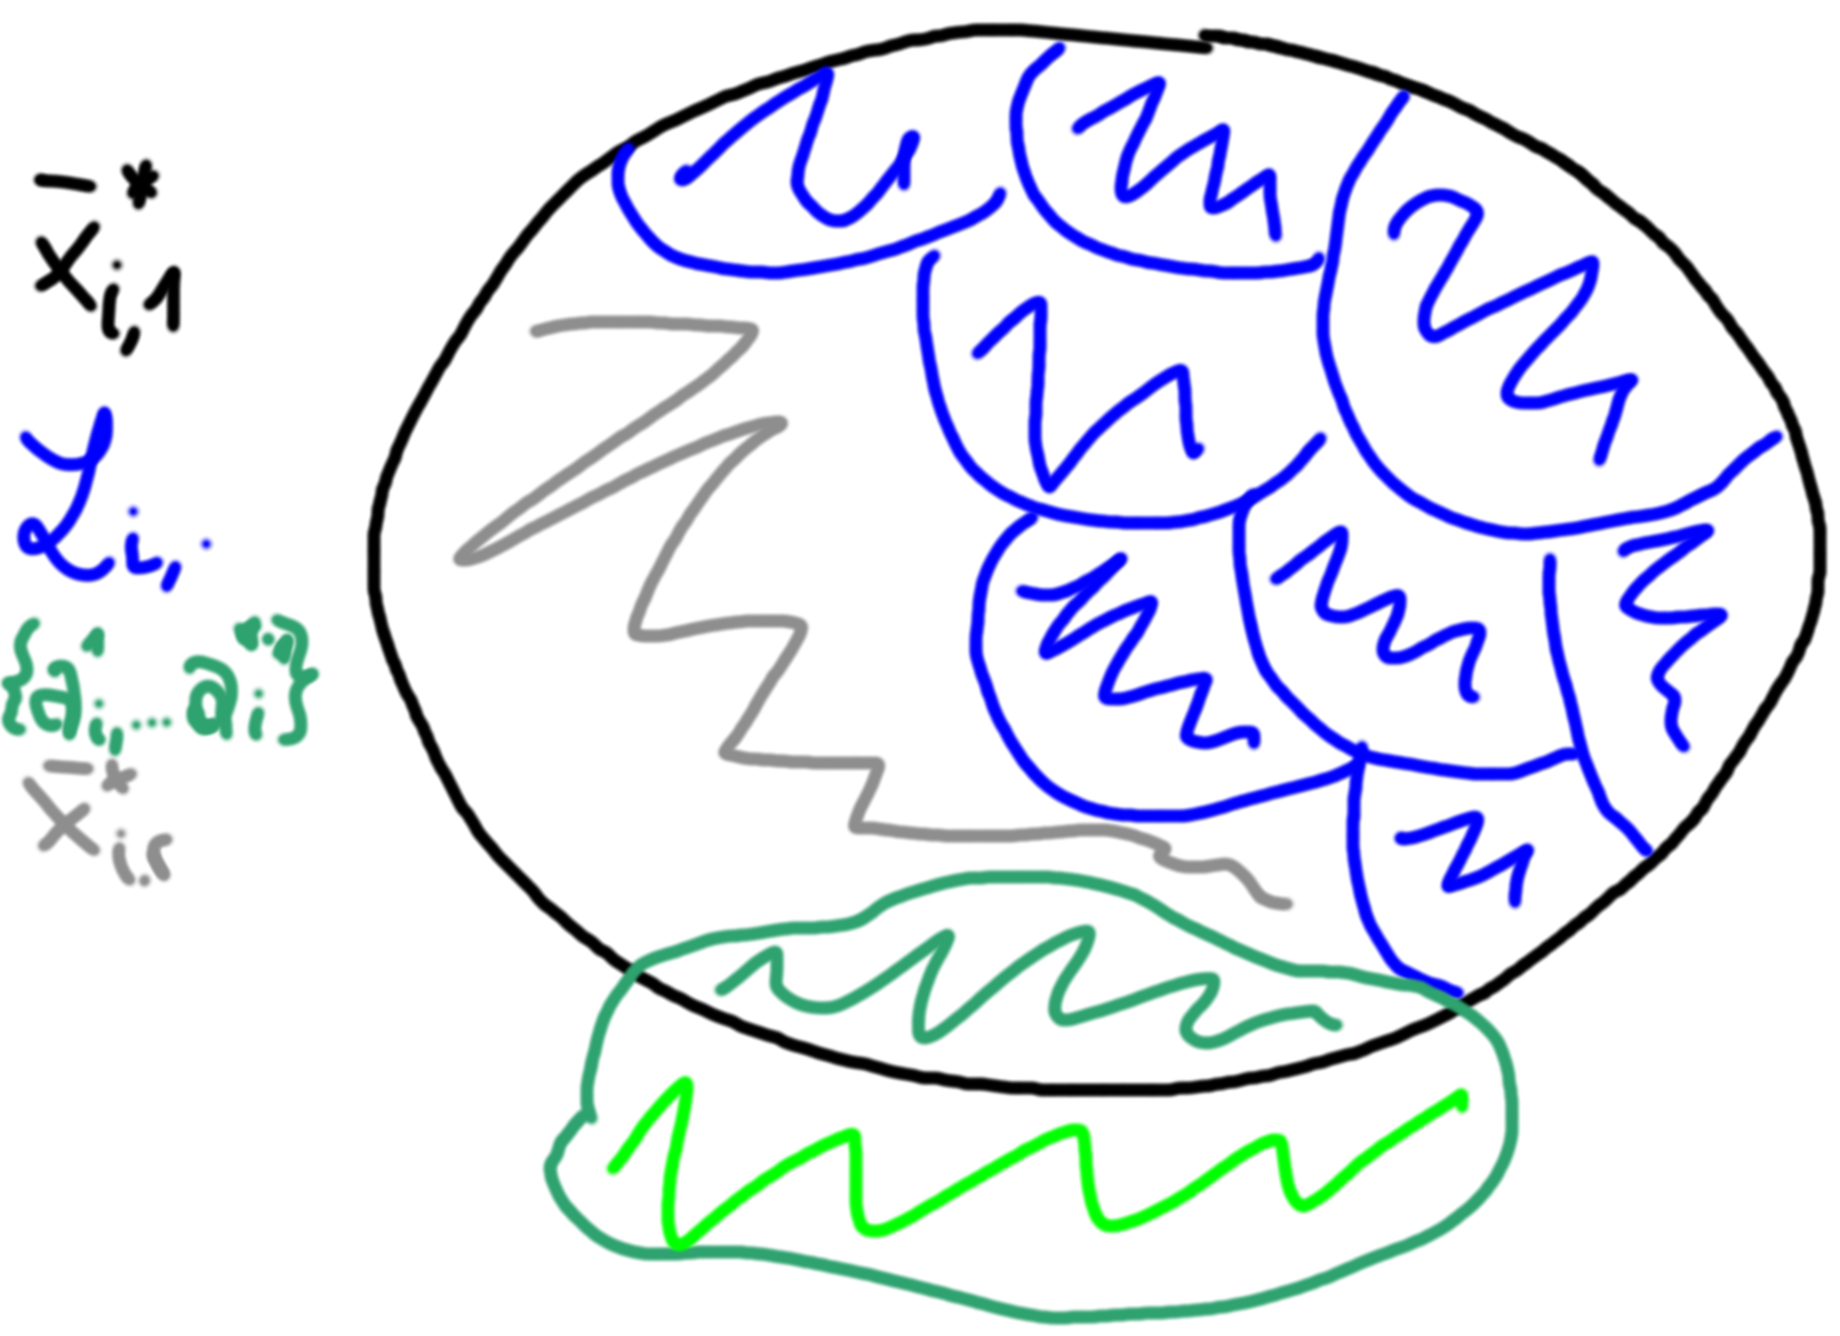
\includegraphics[height=1.45cm]{img/anal2_1}};
	\begin{minipage}{0.66\textwidth}
		\begin{block}{Any Room for Improvement?}
			Possibly! Lower bound of \(1.72\).
		\end{block}
	\end{minipage}
\end{frame}





\begin{frame}[c, plain, noframenumbering]
	\renewcommand{\insertsectionnumber}{!}
	\renewcommand{\insertsection}{End of Talk}
	\sectionpage
\end{frame}